\documentclass{article}

\usepackage{fancyhdr} % Required for custom headers
\usepackage{lastpage} % Required to determine the last page for the footer
\usepackage{extramarks} % Required for headers and footers
\usepackage[usenames,dvipsnames]{color} % Required for custom colors
\usepackage{graphicx} % Required to insert images
\usepackage{listings} % Required for insertion of code
\usepackage{courier} % Required for the courier font
\usepackage{caption}
\usepackage{subcaption}
\renewcommand{\_}{\char`_}

% Margins
\topmargin=-0.45in
\evensidemargin=0in
\oddsidemargin=0in
\textwidth=6.5in
\textheight=9.0in
\headsep=0.25in

\linespread{1.1} % Line spacing

\lstset{language=C,
                basicstyle=\ttfamily,
                keywordstyle=\color{blue}\ttfamily,
                stringstyle=\color{red}\ttfamily,
                commentstyle=\color{Plum}\ttfamily,
                morecomment=[l][\color{magenta}]{\#}
}


% Set up the header and footer
\pagestyle{fancy}
\lhead{Group 18} % Top left header
\chead{Task 1: Scheduling} % Top center head
\rhead{\firstxmark} % Top right header
\lfoot{\lastxmark} % Bottom left footer
\rfoot{Page\ \thepage\ of\ \protect\pageref{LastPage}} % Bottom right footer
\renewcommand\headrulewidth{0.4pt} % Size of the header rule
\renewcommand\footrulewidth{0.4pt} % Size of the footer rule

\setlength\parindent{0pt} % Removes all indentation from paragraphs

%----------------------------------------------------------------------------------------
%	TITLE PAGE
%----------------------------------------------------------------------------------------

\title{
\vspace{2in}
\textmd{\textbf{Task 1: Scheduling}}\\
\normalsize\vspace{0.1in}\small{Due\ on\ Tuesday,\ February\ 9,\ 2016}\\
\vspace{0.1in}\large{\textbf{Pintos Group 18}}
\vspace{3in}
}

\author{Corentin Herbinet, Ignacio Navarro, Vinothan Shankar, William Springsteen}
\date{}

%----------------------------------------------------------------------------------------

\begin{document}

\maketitle
\newpage

\section{Group}

Corentin Herbinet: cah214@ic.ac.uk

Ignacio Navarro

Vinothan Shankar

William Springsteen

\section{Design Questions: Priority Scheduling}
\subsection{Data Structures}
\subsubsection{Purpose of new variables and 'struct' members}

\begin{enumerate}

\item \begin{lstlisting}
struct thread
  {
		.
		.
    struct list locks_holding;           /* List of locks that thread owns. */
    struct lock *waiting_on_lock; 	 /* Lock the thread is waiting on. */ 
    struct semaphore *waiting_on_sema;   /* Semaphore the thread is waiting on. */
		.
		.
  };
\end{lstlisting}

\item \begin{lstlisting}
struct lock 
  {
    struct thread *holder;       /* Thread holding lock (for debugging). */
    struct list_elem lock_elem;  /* For the list of locks a thread has.  */
    struct semaphore semaphore;  /* Binary semaphore controlling access. */
  };
\end{lstlisting}
\end{enumerate}


\begin{enumerate}

\item We have modified \texttt{struct thread} by adding three new members. The first is a list of locks that the thread owns. This 
is useful to modify the effective priority. The second is a pointer to a lock that the thread is waiting on. This pointer is \texttt{NULL}
if the thread is not waiting on any lock. This member is useful to donate priority along the chain. The third is another pointer to a semaphore. This is used in the same manner as the second member but with semaphores, since a thread could be waiting on a semaphore but not on a lock.

\item We have modified only one member in \texttt{struct lock}. This is a \texttt{list\_elem} for the list of locks a thread owns, as explained
in the previous part.
\end{enumerate}

\subsubsection{Data structure used to track priority donation}
To track priority donation we've added a list \texttt{locks\_holding} that each thread has, a lock \texttt{waiting\_on\_lock} that each thread is waiting on (if a thread is not waiting, then this is set to \texttt{NULL}), and a thread \texttt{holder} that each lock has. This is sufficient to track priority donation by the following means. We use two functions \texttt{thread\_donate\_priority(struct thread *donee, int priority)} and \\ \texttt{thread\_recalculate\_priority(struct thread *t)}. The donate function works recursively by donating priority to lower priority threads that have locks a higher priority thread needs access to. Say thread A with higher priority than thread B wants to acquire a lock that thread B owns. Hence in this case the lock's \texttt{holder} would be B, and thread A would set \texttt{waiting\_on\_lock} to point to the lock. Now since A is stuck waiting on thread B, it calls \texttt{lock\_acquire()}, which calls \texttt{sema\_down()}, which itself calls the function \texttt{thread\_donate\_priority(B, A->effective\_priority)}. This function would allow B to have enough priority to run, call \texttt{lock\_release()} to release the lock, and allow A to acquire the lock. When B releases the lock, it calls  \texttt{thread\_recalculate\_priority(B)} which searches through \texttt{locks\_holding} to recalculate the effective priority back so that B, having originally a lower priority, doesn't run. The next example of nested priorities should give a more intuitive feel of how the system works.
\newpage

\begin{figure}[ht!]
\centering
\hspace{3em}
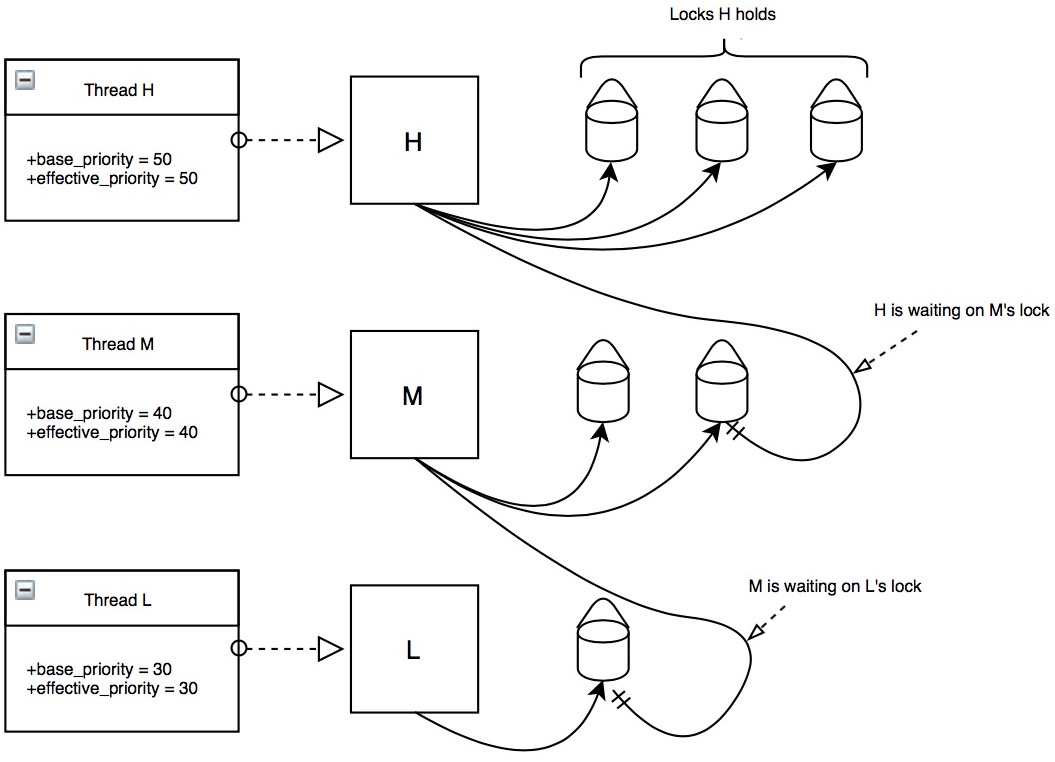
\includegraphics[width=0.6\textwidth]{Images/Task1/1Nested}
\caption{Initial State}
\end{figure}

In the following scenario (Figure 1), thread H is the highest priority thread and therefore in the running state. It currently has three locks, and wants to acquire a fourth by calling \texttt{lock\_acquire()}. If no thread owns the lock (i.e. \texttt{holder} is \texttt{NULL}), then H can acquire the lock. 

\begin{figure}[ht!]
\centering
\hspace{3em}
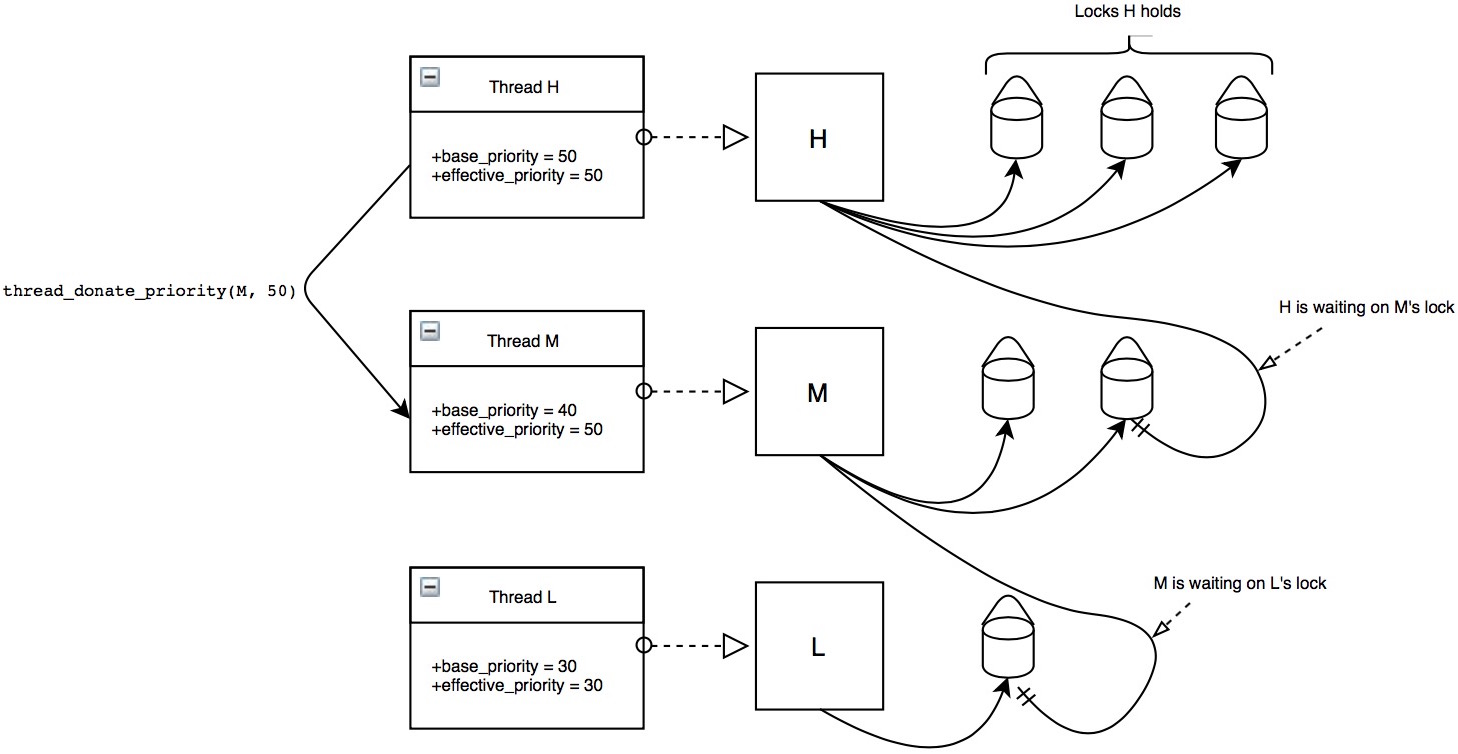
\includegraphics[width=0.8\textwidth]{Images/Task1/2Nested}
\caption{Second State}
\end{figure}

However, M has the lock, so H calls \texttt{thread\_donate\_priority(M, H->effective\_priority)} in Figure 2 so that M can release the lock, recalculate its priority, and H can continue to run. Unfortunately, it is the case that M itself is waiting on another lock L has, so M calls recursively \texttt{thread\_donate\_priority(L, M->effective\_priority)}, as shown in Figure 3.
\newpage

\begin{figure}[ht!]
\centering
\hspace{3em}
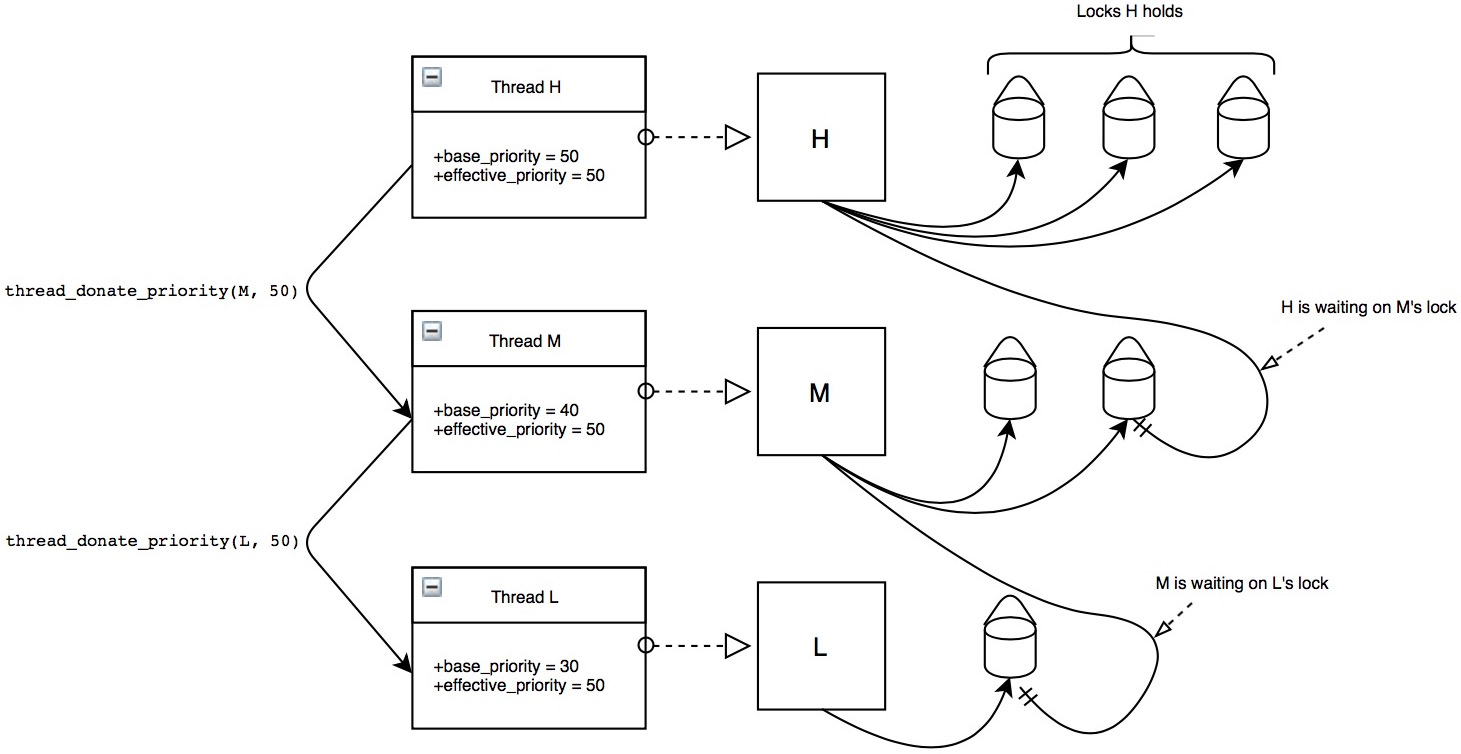
\includegraphics[width=0.8\textwidth]{Images/Task1/3Nested}
\caption{Third State}
\end{figure}

Now L has effective priority 50 and therefore runs. It checks if it is waiting on a lock through \texttt{waiting\_on\_lock}, (it isn't), so we have reached a base case, and \texttt{thread\_donate\_priority(L, M->effective\_priority)} simply returns. L continues to run, and releases the lock it's holding through \texttt{lock\_release()}. This in turn calls \texttt{thread\_recalculate\_priority(L)}, which checks the list of locks L holds \texttt{locks\_holding}. We iterate through all the locks L holds and see for each lock the list of waiting threads on that lock. The highest priority waiting thread would then set the effective priority of L to its effective priority. However, since L is not holding any locks, we simply set the effective priority to the base priority (Figure 4). 

\begin{figure}[ht!]
\centering
\hspace{3em}
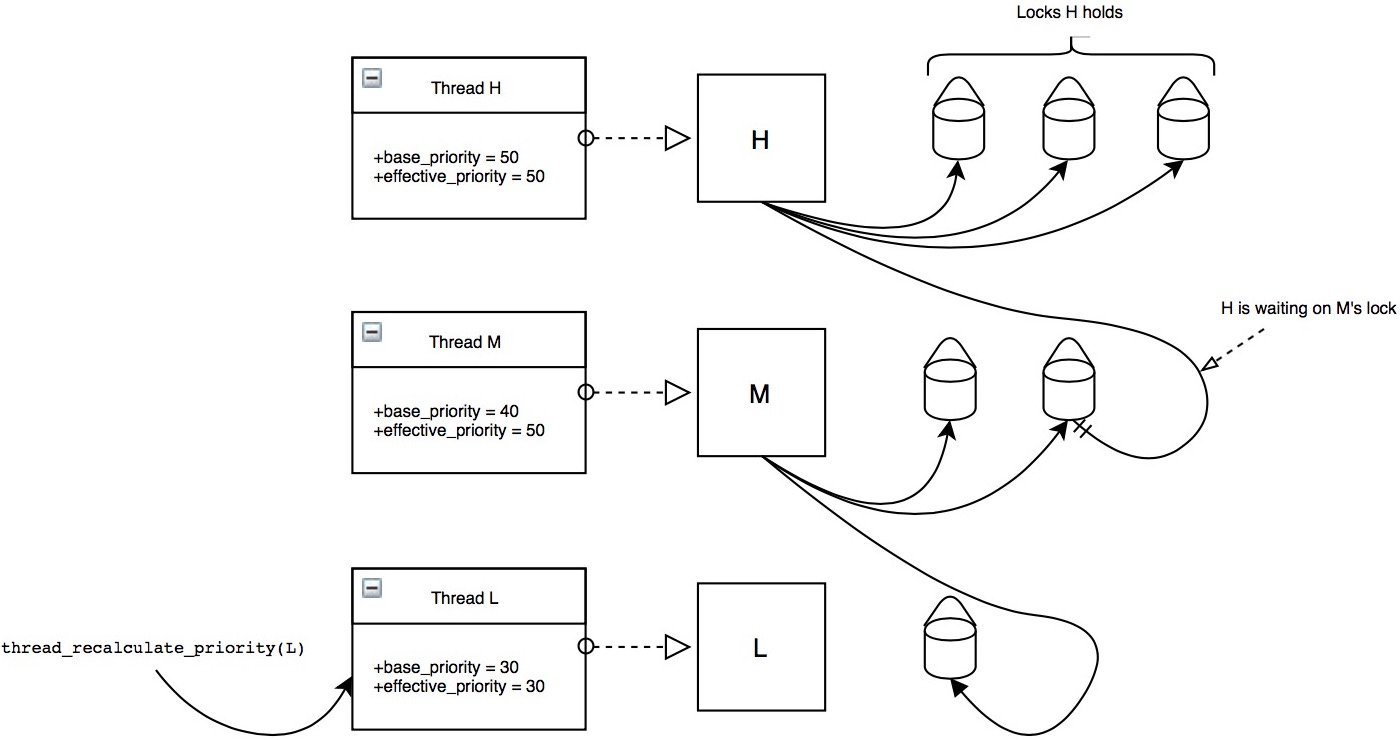
\includegraphics[width=0.8\textwidth]{Images/Task1/4Nested}
\caption{Fourth State}
\end{figure}

Note that in Figure 4 thread L has released the lock, and M is therefore not waiting on any more locks. It would therefore be unblocked and put in a running state. Since M is now running, it can release the lock H wants through \texttt{lock\_release()} which in turn calls \texttt{thread\_recalculate\_priority(M)}. We again iterate through all the locks M holds and see for each lock the list of waiting threads on that lock. The highest priority waiting thread would then set the effective priority of M to its effective priority. However, since M's list of locks have no waiters, we simply set the effective priority to the base priority (Figure 5). 

\begin{figure}[ht!]
\centering
\hspace{3em}
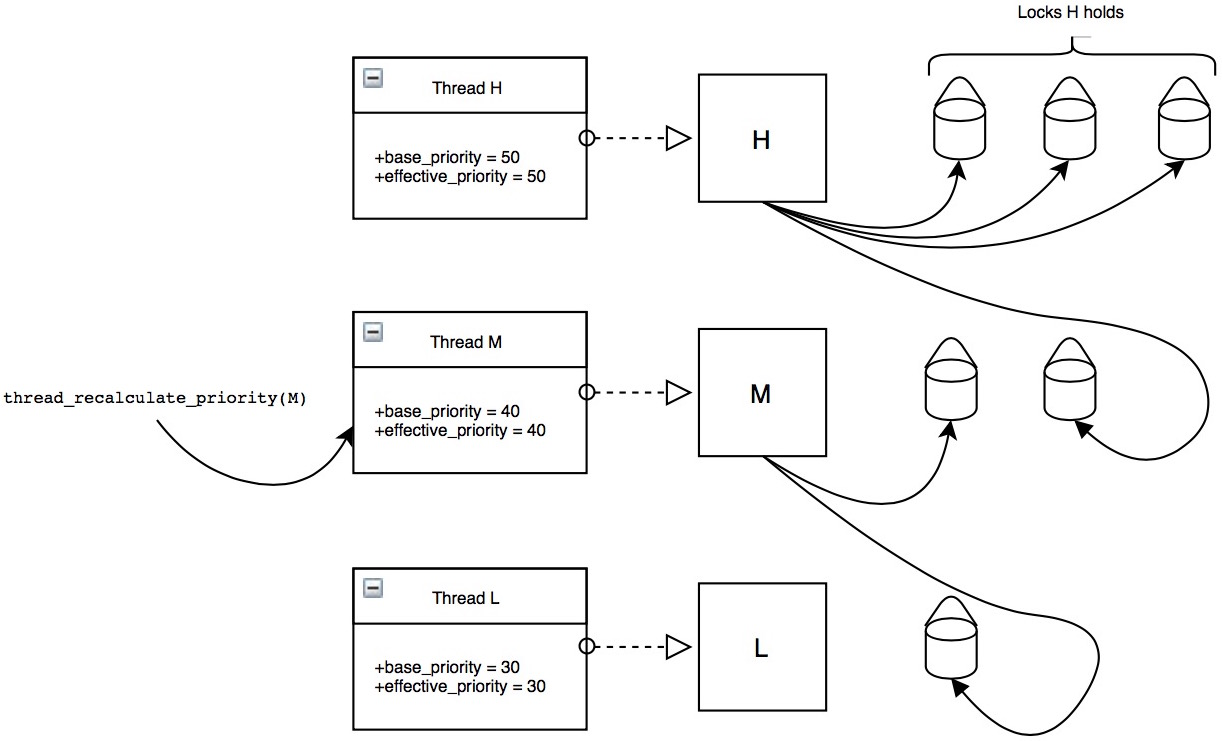
\includegraphics[width=0.8\textwidth]{Images/Task1/5Nested}
\caption{Fifth State}
\end{figure}

Again note how now M has released the lock and set back its effective priority.

\begin{figure}[ht!]
\centering
\hspace{3em}
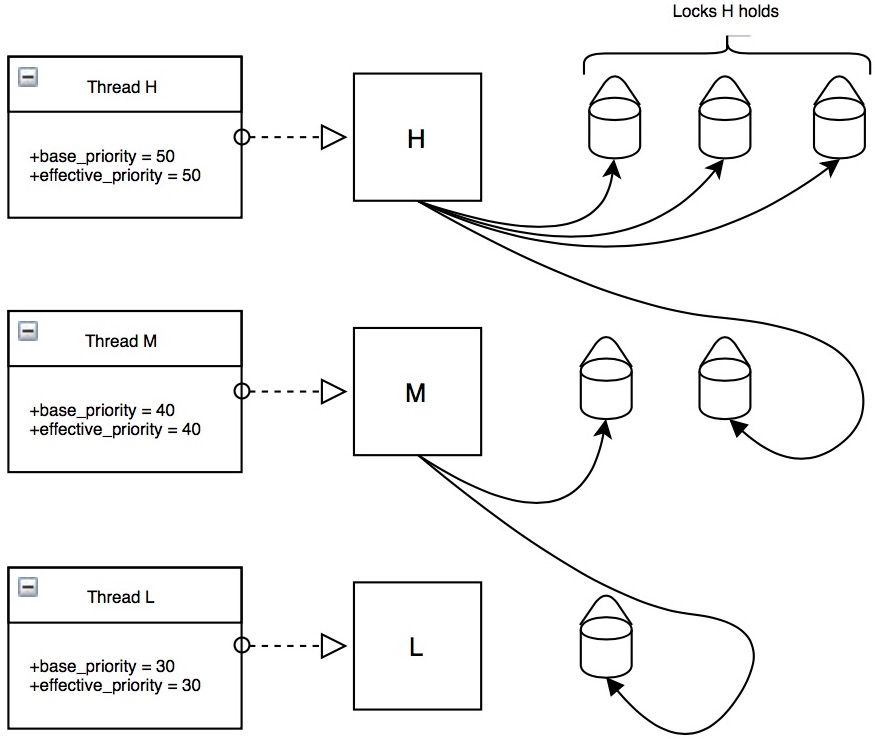
\includegraphics[width=0.6\textwidth]{Images/Task1/6Nested}
\caption{Final State}
\end{figure}

We thus reach our final state, avoiding starvation and deadlock.


%\begin{figure*}
%    \centering
%    \begin{subfigure}[b]{0.50\textwidth}
%   	    \hspace{2em}
%            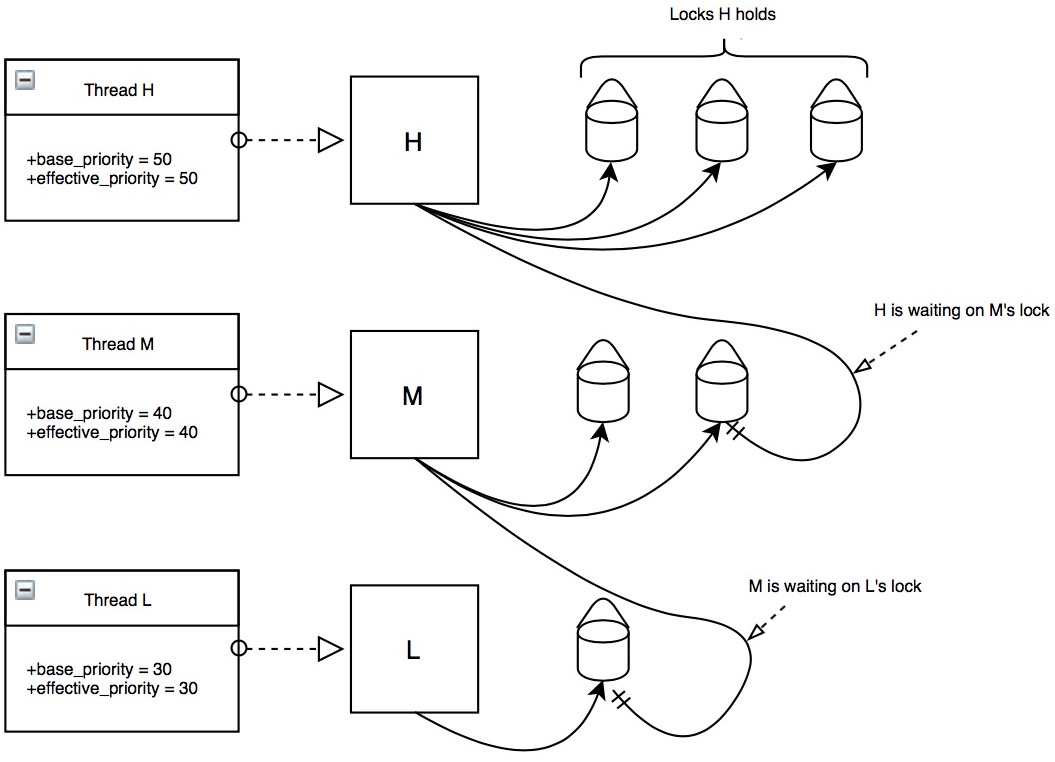
\includegraphics[width=\textwidth]{Images/Task1/1Nested}
%            \caption{Initial State}
%            \label{fig:a}
%    \end{subfigure}
%    
%    \begin{subfigure}[b]{0.49\textwidth}
%            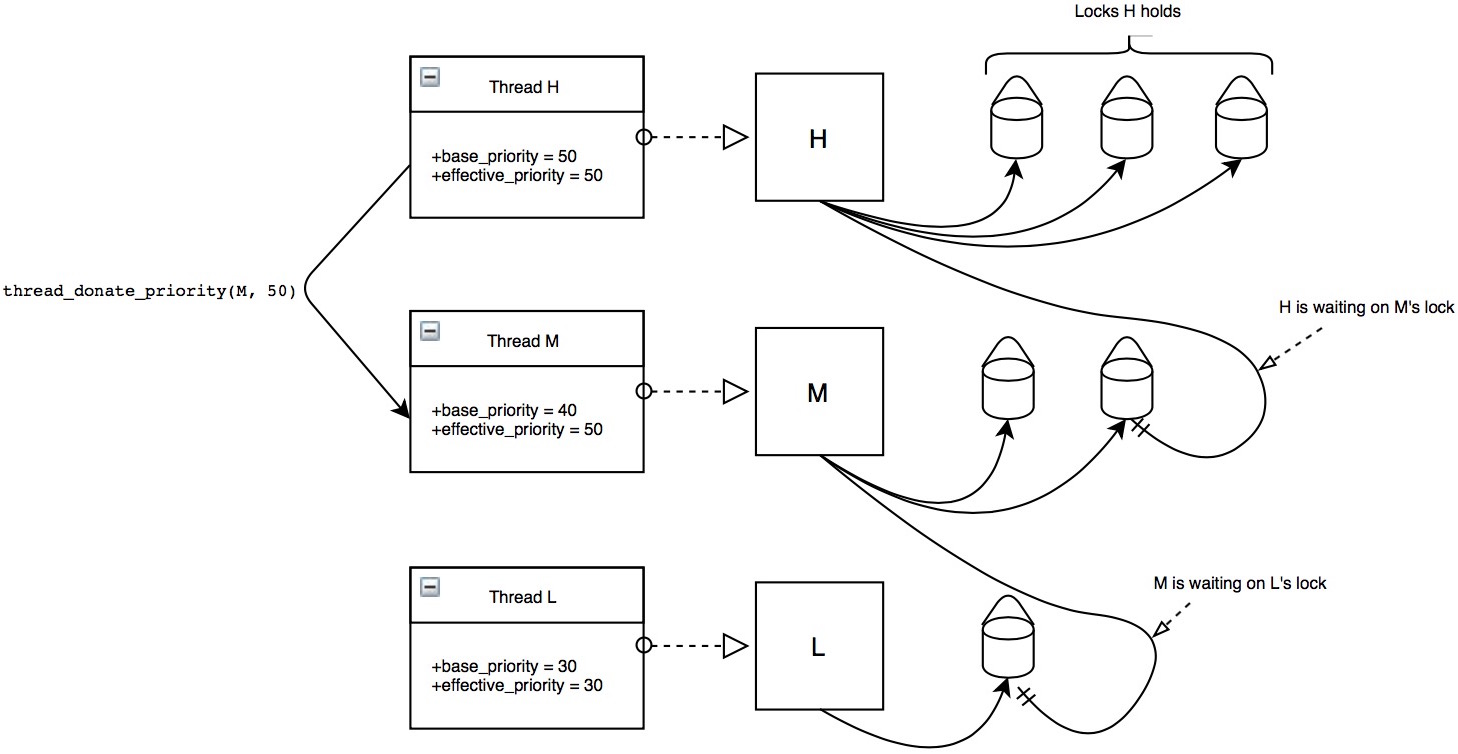
\includegraphics[width=\textwidth]{Images/Task1/2Nested}
%            \caption{c}
%            \label{fig:c}
%    \end{subfigure}
%    % ... this comment too
%    \begin{subfigure}[b]{0.49\textwidth}
%            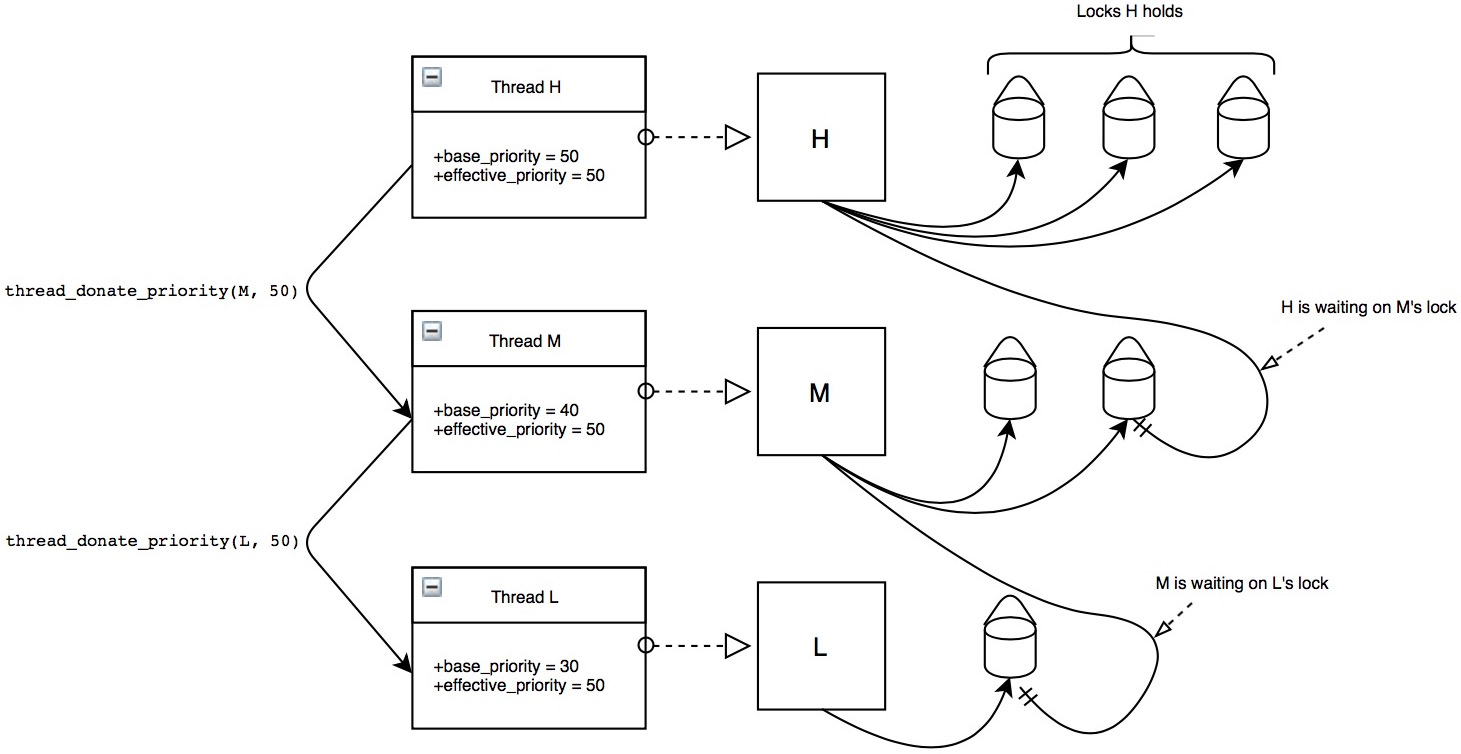
\includegraphics[width=\textwidth]{Images/Task1/3Nested}
%            \caption{d}
%            \label{fig:d}
%    \end{subfigure}
%    \begin{subfigure}[b]{0.49\textwidth}
%            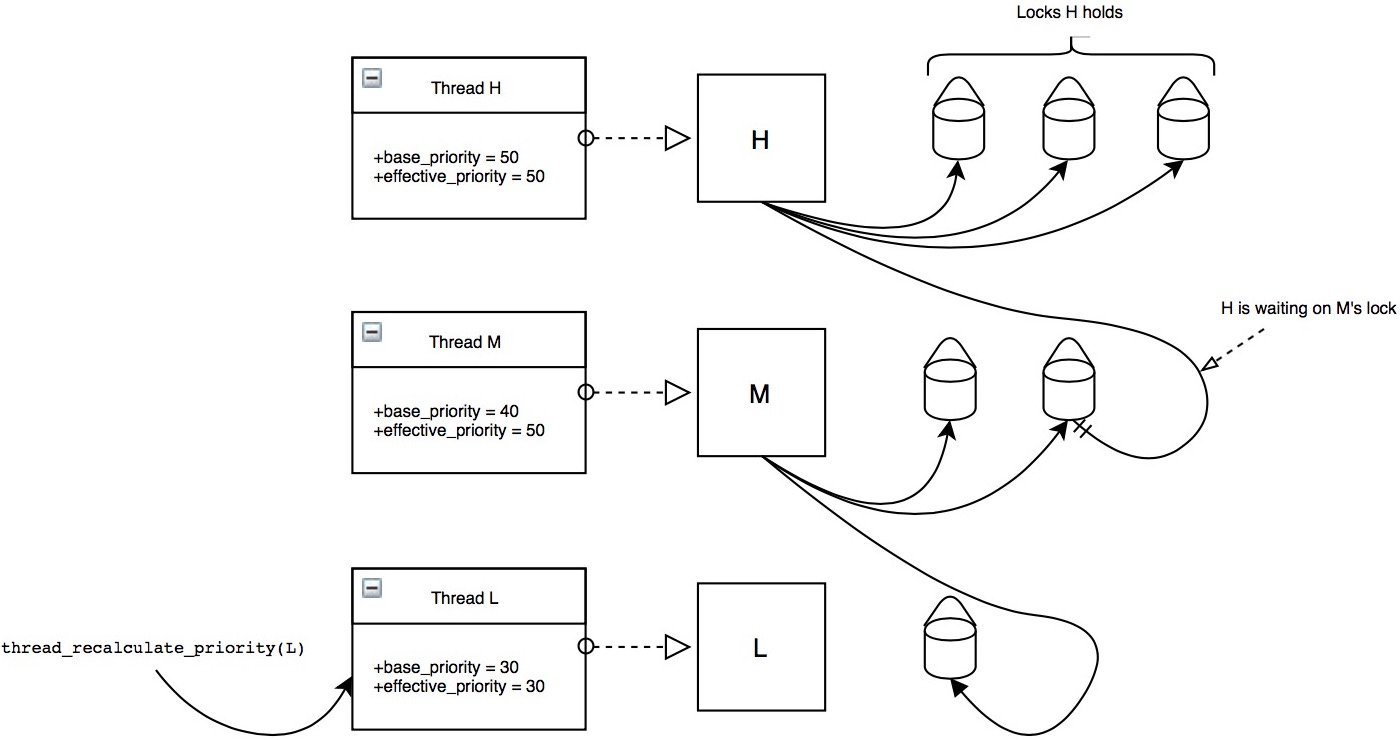
\includegraphics[width=\textwidth]{Images/Task1/4Nested}
%            \caption{c}
%            \label{fig:c}
%    \end{subfigure}
%    % ... this comment too
%    \begin{subfigure}[b]{0.49\textwidth}
%            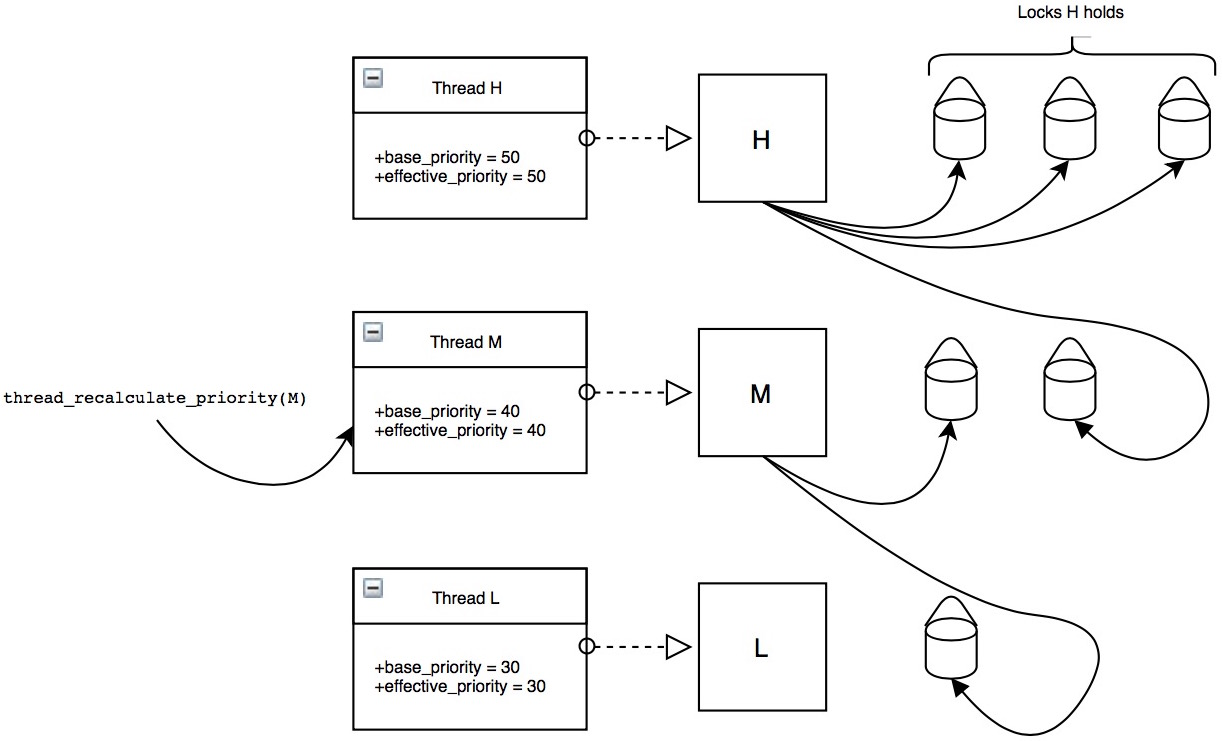
\includegraphics[width=\textwidth]{Images/Task1/5Nested}
%            \caption{d}
%            \label{fig:d}
%    \end{subfigure}
%     \begin{subfigure}[b]{0.50\textwidth}
%            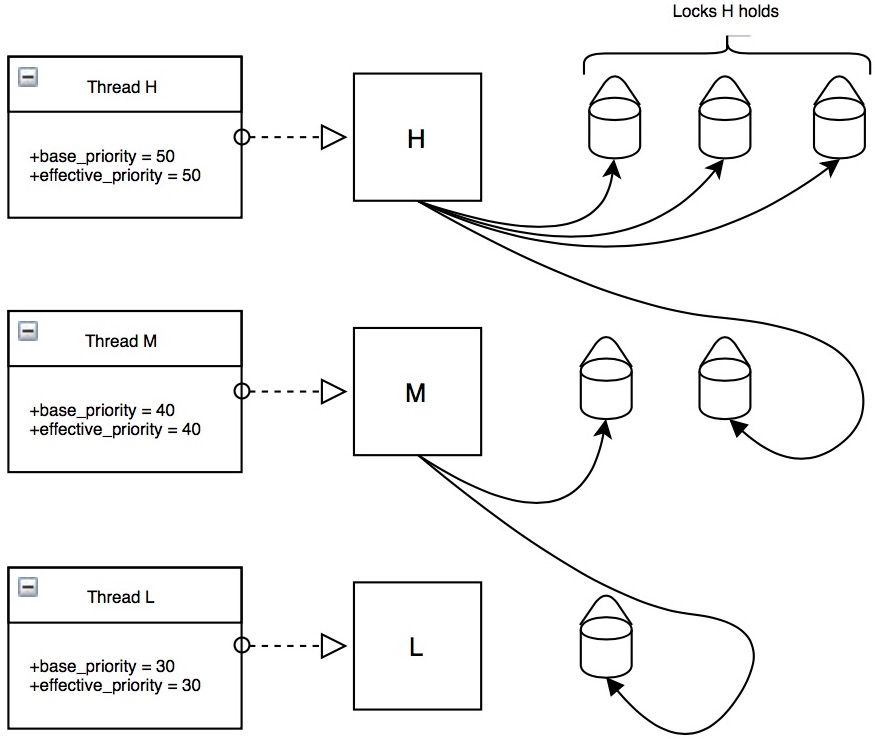
\includegraphics[width=\textwidth]{Images/Task1/6Nested}
%            \caption{Initial State}
%            \label{fig:a}
%    \end{subfigure}
%    \caption{Pictures of ABCD}\label{fig:ABCD}
%\end{figure*}


\subsection{Algorithms}
\subsubsection{Ensuring highest priority thread wakes up first}

To ensure that the highest priority thread waiting for a semaphore wakes up first, we use an ordered list of waiting threads,
in growing order of priority. When \texttt{sema\_down()} is called on a semaphore, the current thread is inserted into the list of waiting threads using the \texttt{less\_priority()} method which compares the priority of two threads. The thread is then blocked while it is waiting for \texttt{sema\_up()} to be called on the semaphore.

Once \texttt{sema\_up()} is called on the semaphore, the last thread in the list of waiting threads, which has the highest priority,
is woken up with \texttt{thread\_unblock()} and removed from the list of waiting threads.

Locks and condition variables both use a semaphore to block and wake up threads: therefore it will use their semaphore's 
ordered list of waiting threads as a way to ensure the highest priority thread will be woken up first, as explained above.

\subsubsection{Sequence of events in \texttt{lock\_acquire()}}

When a call to \texttt{lock\_acquire} causes a priority donation, the following sequence of events happens:

\begin{enumerate}

\item If the lock already has a holder (a thread that is holding the lock), we use the helper method \texttt{thread\_donate\_priority()}, giving it as arguments the thread holding the lock as well as the current thread's priority.

\item If the thread holding the lock has a higher priority than the current thread, the holder continues holding the lock and we return from the method.

\item Otherwise, the current thread's priority becomes the holder's priority.

\item In that case, we check the holder's status: if it is blocked, we remove it from the list of waiting threads and reinsert it in the right order depending on its new priority. If the holder is ready, we remove it from the list of waiting threads and add it to the list of threads ready to run.

\item Finally, if the holder of the lock (Lock A) is waiting for another lock (Lock B) to be released, we call \texttt{thread\_donate\_priority()} with Lock B's holder and Lock A's holder's new priority: this helper method therefore works recursively in the case of nested priority donation.

\item We then leave the helper method, and call \texttt{sema\_down()} on the lock's semaphore.

\end{enumerate}

\subsubsection{Sequence of events in \texttt{lock\_release()}}

When \texttt{lock\_release()} is called on a lock that a higher priority thread is waiting for, the following sequence of events happens:

\begin{enumerate}

\item The lock's holder is set to NULL.

\item The lock is removed from the list of locks the current thread is holding.

\item We call a helper method \texttt{thread\_recalculate\_effective\_priority()} on the current thread: if the current thread does not hold any other locks, it takes back its base priority value and the method returns. Otherwise, it traverses through the list of locks it is holding, setting its effective priority to the largest effective priority out of the effective priorities of the lock's waiters.

\item In that case, if the current thread's effective priority is lower than the highest available priority found in the previous traversal, the thread yields.

\item Finally, we leave the helper method and \texttt{sema\_up()} is called on the lock's semaphore.

\end{enumerate}

\subsection{Synchronization}
\subsubsection{Potential race in \texttt{thread\_set\_priority()}}

\subsection{Rationale}

\subsubsection{Choice of design and superiority to other designs}

\newpage

\section{Design Questions: Advanced Scheduler}
\subsection{Data Structures}
\subsubsection{Purpose of new variables}

\subsection{Algorithms}
\subsubsection{Table}
\subsection{Ambiguities in scheduler specification and resolution}
\subsubsection{Dividing cost of scheduling}

\subsection{Rationale}
\subsubsection{Critique of design}

\subsubsection{Design in fixed-point arithmetic}


%----------------------------------------------------------------------------------------

\end{document}